\let\negmedspace\undefined
\let\negthickspace\undefined
\documentclass[journal]{article}
\usepackage[a5paper, margin=10mm, onecolumn]{geometry}
\usepackage{lmodern} % Ensure lmodern is loaded for pdflatex

\setlength{\headheight}{1cm} % Set the height of the header box
\setlength{\headsep}{0mm}     % Set the distance between the header box and the top of the text

\usepackage{gvv-book}
\usepackage{gvv}
\usepackage{cite}
\usepackage{textcomp}
\usepackage{amsmath,amssymb,amsfonts,amsthm}
\usepackage{algorithmic}
\usepackage{graphicx}
\graphicspath{{./figs/}}
\usepackage{textcomp}
\usepackage{xcolor}
\usepackage{txfonts}
\usepackage{listings}
\usepackage{enumitem}
\usepackage{mathtools}
\usepackage{gensymb}
\usepackage{comment}
\usepackage[breaklinks=true]{hyperref}
\usepackage{tkz-euclide} 
\usepackage{listings}
\usepackage{gvv}                                        
\def\inputGnumericTable{}                                 
\usepackage[latin1]{inputenc}                                
\usepackage{color}                                            
\usepackage{array}                                            
\usepackage{longtable}                                       
\usepackage{calc}                                             
\usepackage{multirow}                                         
\usepackage{hhline}                                           
\usepackage{ifthen}                                           
\usepackage{lscape}
\usepackage{circuitikz}
\tikzstyle{block} = [rectangle, draw, fill=blue!20, 
text width=4em, text centered, rounded corners, minimum height=3em]
\tikzstyle{sum} = [draw, fill=blue!10, circle, minimum size=1cm, node distance=1.5cm]
\tikzstyle{input} = [coordinate]
\tikzstyle{output} = [coordinate]


\begin{document}
	
	\bibliographystyle{IEEEtran}
	\vspace{3cm}
	
\title{4.3.37}
\author{EE25BTECH11047 - RAVULA SHASHANK REDDY}
\maketitle
\hrulefill
\bigskip 

\renewcommand{\thetable}{\theenumi}
\setlength{\intextsep}{10pt}

\textbf{Question:}  
Find the equation of the line passing through the points  
\[
\vec{A} = \myvec{1 \\ 2}, 
\quad 
\vec{B} = \myvec{3 \\ 6}.
\]

\textbf{Solution:}  

\begin{align}
\myvec{\vec{A}&\vec{B}}^T\vec{n} &= \myvec{1\\1}\\
\myvec{1 & 2 \\ 3 & 6}\vec{n} &= \myvec{1 \\ 1}\\ 
\myvec{1 & 2 & 1 \\ 3 & 6 & 1} & 
\xrightarrow{R_2 - 3R_1}\;\;
\myvec{1 & 2 & 1 \\ 0 & 0 & -2} \\
0=-2
\end{align}
\begin{center}
Inconsistent.Hence c=0.
\end{center}
\begin{align}
\myvec{1 & 2 \\ 3 & 6}\vec{n} &= \myvec{0 \\ 0} 
\end{align}
\begin{align}
\myvec{1 & 2 & 0 \\ 3 & 6 & 0} & 
\xrightarrow{R_2 - 3R_1}\;\;
\myvec{1 & 2 & 0 \\ 0 & 0 & 0} 
\end{align}

\begin{align}
\vec{n} &= \myvec{-2 \\ 1}
\end{align}

Equation of a Line is
\begin{align}
\vec{n}^T \vec{x} &= c \\
\myvec{-2 & 1}\myvec{1 \\ 2} &= c \\
c &= 0 \\
\myvec{-2 & 1}\vec{x} &= 0 \\
-2x + y &= 0 \\
\boxed{y = 2x}
\end{align}
\newpage
\begin{figure}
    \centering
    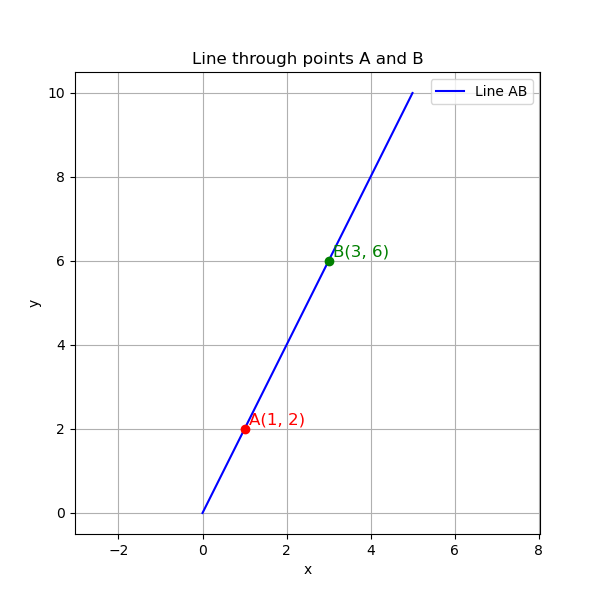
\includegraphics[width=1.0\linewidth]{figs/fig1.png}
    \caption{Caption}
    \label{fig:placeholder}
\end{figure}
\end{document}